\documentclass[tikz, preview]{standalone}

\usepackage{tikz}
\usepackage[all,2cell]{xy}
\usetikzlibrary{matrix,arrows,shapes,decorations.markings}
\definecolor{rewritecolor}{rgb}{0,.9,1}
\tikzset{rewritenode/.style={shape=circle,fill=rewritecolor,scale=0.25,font=\Huge}}
\tikzset{RWopen/.style={shape=circle,draw=black,thick,fill=white,scale=0.5,font=\Huge}}
\tikzset{RWclosed/.style={shape=circle,thick,fill=black,scale=0.5,font=\Huge}}
\tikzset{CDnode/.style={shape=circle,fill=white,scale=.5}}
\tikzset{zxgreen/.style={shape=circle,thick,draw,fill=green}}
\tikzset{zxred/.style={shape=circle,draw,thick,fill=red}}
\tikzset{zxyellow/.style={shape=rectangle,draw,thick,fill=yellow}}
\tikzset{zxdiamond/.style={shape=diamond,fill=black,inner sep=2.75}}
\tikzset{zxopen/.style={shape=circle,draw,thick,inner sep=2pt}}
\tikzset{->-/.style={decoration={markings,mark=at position .5 with {\arrow{>}}},postaction={decorate}}}
\tikzset{->-pos/.style={decoration={markings,mark=at position #1 with {\arrow{>}}},postaction={decorate}}}

\begin{document}

\[
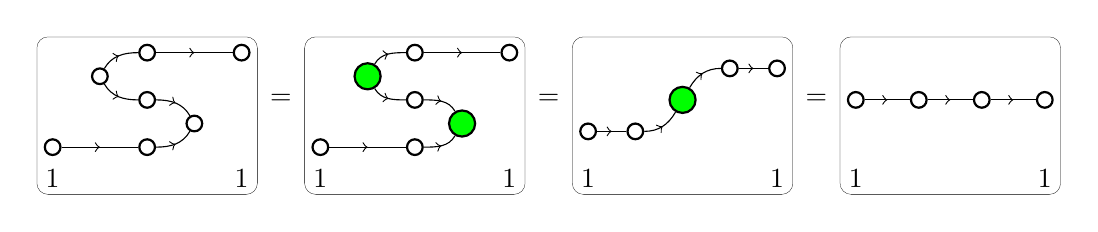
\begin{tikzpicture}
%
% SCOPE 1
%
\begin{scope}[shift={(0.4,0)}]
\node [zxopen] (o1) at (0,0) {};
\node [zxopen] (o2) at (-0.6,-0.3) {};
\node [zxopen] (o3) at (0,-0.6) {};
\node [zxopen] (o4) at (0.6,-0.9) {};
\node [zxopen] (o5) at (0,-1.2) {};
\node [zxopen] (in1) at (-1.2,-1.2) {};
\node [zxopen] (out1) at (1.2,0) {};
%
\draw [->-]  (in1) to (o5);
\draw [->-] (o2) to [out=60,in=180] (o1);
\draw [->-] (o2) to [out=-60,in=180] (o3);
\draw [->-]  (o5) to [out=0,in=-120] (o4);
\draw [->-]  (o3) to [out=0,in=120] (o4);
\draw [->-] (o1) to (out1);
%
\node (r1) at (-1.4,0.2) {};
\node (r2) at (1.4,-1.8) {};
\draw [rounded corners, ultra thin] (r1) rectangle (r2);
%
\node at (-1.2,-1.6) {$1$};
\node at (1.2,-1.6) {$1$};
\end{scope}
%
% SCOPE 2
%
\begin{scope}[shift={(3.8,0)}]
\node [zxopen] (o1) at (0,0) {};
\node [zxopen] (o2) at (0,-0.6) {};
\node [zxopen] (o3) at (0,-1.2) {};
\node [zxopen] (in1) at (-1.2,-1.2) {};
\node [zxopen] (out1) at (1.2,0) {}; 
\node [zxgreen] (g1) at (-0.6,-0.3) {};
\node [zxgreen] (g2) at (0.6,-0.9) {};
%
\draw [->-] (g1) to [out=60,in=180] (o1);
\draw [->-] (g1) to [out=-60,in=180] (o2);
\draw [->-]  (o3) to [out=0,in=-120] (g2);
\draw [->-]  (o2) to [out=0,in=120] (g2);
\draw [->-] (o1) to (out1);
\draw [->-]  (in1) to (o3);
%
\node (r1) at (-1.4,0.2) {};
\node (r2) at (1.4,-1.8) {};
\draw [rounded corners, ultra thin] (r1) rectangle (r2);
%
\node at (-1.2,-1.6) {$1$};
\node at (1.2,-1.6) {$1$};
\end{scope}
%
% SCOPE 3
%
\begin{scope}[shift={(7.2,0)}]
\node [zxopen] (o1) at (0.6,-0.2) {};
\node [zxopen] (o2) at (-0.6,-1) {};
\node [zxopen] (in1) at (-1.2,-1) {};
\node [zxopen] (out1) at (1.2,-0.2) {}; 
\node [zxgreen] (g1) at (0,-0.6) {};
%
\draw [->-] (g1) to [out=60,in=180] (o1);
\draw [->-]  (o2) to [out=0,in=-120] (g1);
\draw [->-] (o1) to (out1);
\draw [->-]  (in1) to (o2);
%
\node (r1) at (-1.4,0.2) {};
\node (r2) at (1.4,-1.8) {};
\draw [rounded corners, ultra thin] (r1) rectangle (r2);
%
\node at (-1.2,-1.6) {$1$};
\node at (1.2,-1.6) {$1$};
\end{scope}
%
% SCOPE 3
%
\begin{scope}[shift={(10.6,0)}]
\node [zxopen] (o1) at (0.4,-0.6) {};
\node [zxopen] (o2) at (-0.4,-0.6) {};
\node [zxopen] (in1) at (-1.2,-0.6) {};
\node [zxopen] (out1) at (1.2,-0.6) {}; 
%
\draw [->-] (o2) to (o1);
\draw [->-] (o1) to (out1);
\draw [->-]  (in1) to (o2);
%
\node (r1) at (-1.4,0.2) {};
\node (r2) at (1.4,-1.8) {};
\draw [rounded corners, ultra thin] (r1) rectangle (r2);
%
\node at (-1.2,-1.6) {$1$};
\node at (1.2,-1.6) {$1$};
\end{scope}
%
% EQUAL SIGNS
%
\node at (2.1,-0.6) {$=$};
\node at (5.5,-0.6) {$=$};
\node at (8.9,-0.6) {$=$};
%
%
%
\end{tikzpicture}
\]



\end{document}
